Without loss of generality, let us focus on one particular source of uncertainty: the subthreshold leakage current and, more specifically, on the effective channel length.
The reason for this choice is that the effective channel length has the strongest influence on leakage \cite{chandrakasan2001, srivastava2010, juan2011, juan2012}; in particular, it also affects the threshold voltage. Consequently, in what follows, $\u$ stands for this crucial parameter.

Now we shall describe the default configuration of our experimental setup, which, in the following subsections, will be adjusted according to the purpose of each particular experiment.
We consider a 45-nanometer technological process. The diameter of the wafer is 20 dies, the total number of dies $\ndies$ is 316, and the number of processing elements $\nprocs$ in each of the dies is four.
The number of measured dies $\nrdies$ is 20. These dies are chosen as follows: the first one is placed in the middle of the wafer, and the other are selected sequentially such that the total distance from the already picked dies and the new one to the rest of the dies is minimized.
The floorplans of the multiprocessor platforms are constructed in such a way that the processing elements form regular grids, as it is the case with, \eg, Alpha 21264 studied in \cite{juan2011}. The capacitance and conductance matrices in \eref{heat-de} are obtain using HotSpot v5.02 \cite{hotspot}.
The dynamic power profiles involved in the experiments are based on simulations of randomly generated (via TGFF v3.5 \cite{dick1998}) task graphs.\footnote{The floorplans of the platforms, thermal configuration of HotSpot, task graphs of the applications, \etc\ are available online at \cite{sources}.} The sampling interval of power profiles is $1~\text{ms}$.
Without loss of generality, the temperature- and channel-length-aware leakage model, used as a part of the power model given by \eref{total-power}, is constructed via SPICE simulations of reference electrical circuits built with the Predictive Technology Model \cite{ptm}, which is followed by a curve fitting procedure.
The corresponding temperature profiles that form the input data set $\Data$ are obtained as follows: (a) draw a sample of $\u$ from a Gaussian distribution with mean $45~\text{nm}$ and the covariance function given by \eref{covariance-function} wherein the standard deviation is $5\%$ \cite{juan2011, juan2012}; (b) simulate the thermal system in \eref{thermal-system} once for each of the $\nrdies$ selected dies using the input dynamic power profile $\profilePdyn$; (c) shrink the full temperature profiles to keep only $\nrsteps$, which is equal to 20 by default, evenly spaced moments of time; and (d) perturb the obtained data using a white Gaussian noise with the standard deviation of $1~\text{K}$ (Kelvin).

Let us turn to the statistical model in \sref{statistical-model} and summarize the intuition and our assignment for each parameter of this model.
In the covariance function given by \eref{covariance-function}, the weight parameter $\eta$ and the two length-scale parameters $\ell_\SE$ and $\ell_\OU$ should be set according to the correlation patterns typical for the production process at hand \cite{chandrakasan2001, cheng2011} (recall the explanation below \eref{covariance-function}); we set $\eta$ to 0.7 and $\ell_\SE$ and $\ell_\OU$ to half the radius of the wafer.
The threshold parameter of the model order reduction procedure described in \aref{kl-expansion} and utilized in \eref{kl-approximation} should be set high enough to preserve a sufficiently large portion of the variance of the data and, thus, to keep the corresponding results accurate; we set it to $0.99$ preserving $99\%$ of this variance. The resulting dimensionality $\nvars$ of $\vz$ in \eref{kl-approximation} was found to be 27--28.
The parameters $\mu_0$ and $\tau_\u$ of the priors in \eref{mu-u-prior} and \eref{sigma2-u-prior} are specific to the considered technological process; we set $\mu_0$ to $45~\text{nm}$ and $\tau_\u$ to $5\%$ of $\mu_0$ \cite{juan2011, juan2012}.
The parameters $\sigma_0$ and $\nu_\u$ determine the precision of the information on $\mu_0$ and $\tau_\u$ and are set according to the beliefs of the user; we set $\sigma_0$ to $1\%$ of $\mu_0$ and $\nu_\u$ to ten.
The latter can be thought of as the number of imaginary observations that the choice of $\tau_\u$ is based on.
In \eref{sigma2-noise-prior}, the parameter $\tau_\noise$ represents the precision (deviation) of the equipments utilized to collect the temperature measurements in the data set $\Data$ and can be found in the technical specification of these equipments; we set $\tau_\noise$ to $1~\text{K}$. The parameter $\nu_\noise$ has the same interpretation as $\nu_\u$; we set it to ten as well.
In \eref{proposal}, $\nu$ and $\alpha$ are tuning parameters, which can be configured based on experiments; we set $\nu$ to eight and $\alpha$ to 0.5.
The number of sample draws is another tuning parameter, which we set to $10^4$; the first half of these samples is ascribed to the burn-in period leaving $5 \cdot 10^3$ effective samples $\nsamples$.
For the proposal optimization in \sref{optimization}, we use the Quasi-Newton algorithm \cite{press2007}.
For parallel computing, we utilize four processors. All the experiments have been conducted on a GNU/Linux machine with Intel Core i7 2.66~GHz and 8~GB of RAM.

\subsection{Analysis of the Experimental Setup}
\begin{figure}[b]
  \centering
  \vspace{-1.5em}
  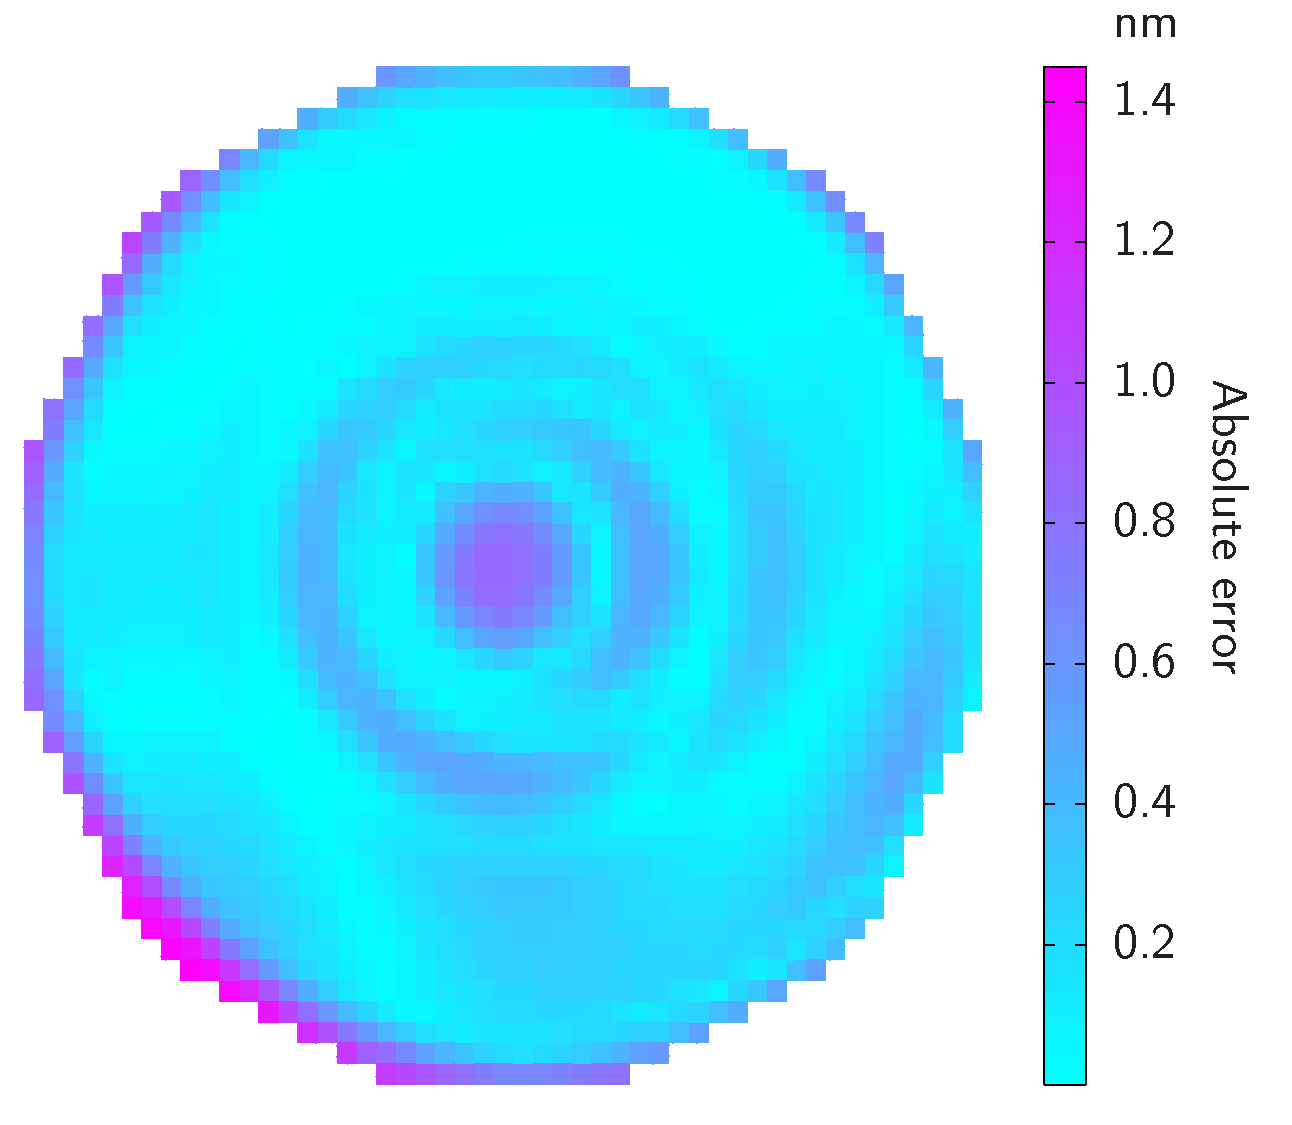
\includegraphics[width=0.6\linewidth]{include/figures/wafer-qoi-error.pdf}
  \caption{Distribution of the absolute error.}
  \flabel{wafer-qoi-error}
\end{figure}

In order to ensure that the experimental setup is adequate, let us first perform a detailed analysis of the results obtained for one particular example with the default configuration described earlier.
The true and inferred distributions of the \qoi\ are shown in \fref{wafer-qoi} where the normalized root-mean-square error (NRMSE) is below $2.8\%$, and the distribution of the absolute error across the wafer is visualized in \fref{wafer-qoi-error}. It can be seen that the framework produces a close match to the true value of the \qoi.
Next we inspect the trace of the obtained sequence of samples and observe that the constructed Markov chain vividly explores the underlying probability space.
Another test commonly used to assess the quality of the proposal distribution is to compare the posterior in \eref{posterior} with the tailored proposal distribution in \eref{proposal} for each parameter conditioned on the other parameters being at $\hat{\vparam}$ (see \sref{optimization}).
The two are found to be practically indistinguishable implying a high quality of the proposal.
To sum up, the performed analysis suggests that the optimization and sampling procedures are fine-tuned.
In what follows, we shall use the assessed default configuration and alter only one parameter at a time: the number of processing elements on a die $\nprocs$, the number of measured dies on the wafer $\nrprocs$, the number of temporal measurements $\nrsteps$, and the deviation of the noise $\sigma_\noise$.

\subsection{Number of Processing Elements on a Die}
In this subsection, we consider five platforms with the number of processing elements in each die $\nprocs$ equal to 2, 4, 8, 16, and 32, respectively. The results are summarized in \tref{processing-elements}.
In this and the following tables, we report the optimization (Stage~2 in \fref{algorithm}) and sampling (Stage~3 in \fref{algorithm}) times separately (given in minutes); moreover, the sampling time is given for two cases: sequential and parallel computing, which is followed by the total time and error (NRMSE). The computational time of the post-processing phase (Stage~4 in \fref{algorithm}) is not given as it is negligibly small.
The sequential sampling time is the most representative indicator of the computational complexity scaling as the number of samples is always fixed, and there is no parallelization; thus, we shall watch this value in most of the discussions below (highlighted in bold in the tables). The speedup due to parallel computing will be discussed later on.
\begin{table}[h]
  \centering
  \caption{Results for the number of processors $\nprocs$.}
  \begin{tabular*}{1\linewidth}{=l@{\hskip 4em}-r-r-r-r-r}
    \toprule
    Processing elements    & 2 & 4 & 8 & 16 & 32 \\
    \midrule
    \midrule
    Optimization time, m   & 2.67 & 3.34 &  5.20 &  7.37 & 13.85 \\
    \midrule
    \rowstyle{\bfseries}
    Sequential sampling, m & 3.71 & 4.60 &  6.03 &  8.92 & 14.77 \\
    Total time, m          & 6.38 & 7.94 & 11.23 & 16.29 & 28.62 \\
    \midrule
    Parallel sampling, m   & 0.98 & 1.18 &  1.58 &  2.51 & 5.30 \\
    Total time, m          & 3.65 & 4.52 &  6.78 &  9.88 & 19.15 \\
    \midrule
    NRMSE, \%              & 4.71 & 3.42 &  3.68 &  2.73 &  1.94 \\
    \bottomrule
  \end{tabular*}
  \tlabel{processing-elements}
  \vspace{-1em}
\end{table}


It can be seen in \tref{processing-elements} that all computational times grow with the number of processing elements. This behavior is expected as each processing element introduces additional complexity in the thermal system given by \eref{thermal-system}. More precisely, it leads to a larger number of thermal nodes $\nnodes$. Nevertheless, even for large examples, the timing is readily acceptable, taking into account the complexity of the inference procedure behind and the yielded accuracy.
An interesting observation can be made from the NRMSE: the error tends to decrease as the number of processing elements grows. The explanation is that, with each processing element, $\Data$ delivers more information to the inference to work with since the temperature profiles in $\Data$ are collected for all processing elements simultaneously; recall that, in our scenario (\sref{model-order-reduction}), the user is assumed to be interested in all processing elements on the die, \ie, $\nrprocs = \nprocs$ in \fref{wafer-measured}.

\subsection{Number of Measured Dies}
\begin{table}[h]
  \centering
  \caption{Results for the number of measured dies.}
  \begin{tabular*}{1\linewidth}{=l@{\hskip 4pt}-r-r-r-r-r-r}
    \toprule
    Measured dies   & 1 & 10 & 20 & 40 & 80 & 160 \\
    \midrule
    \midrule
    Optimization time, m   &  0.41 & 2.49 & 3.34 &  4.59 &  7.33 & 10.29 \\
    \midrule
    \rowstyle{\bfseries}
    Sequential sampling, m &  2.40 & 3.99 & 4.60 &  5.79 &  8.49 & 12.96 \\
    Total time, m          &  2.81 & 6.47 & 7.94 & 10.38 & 15.81 & 23.25 \\
    \midrule
    Parallel sampling, m   &  0.61 & 1.02 & 1.18 &  1.51 &  2.16 &  3.62 \\
    Total time, m          &  1.02 & 3.50 & 4.52 &  6.10 &  9.49 & 13.91 \\
    \midrule
    NRMSE, \%              & 30.49 & 4.40 & 3.42 &  1.09 &  0.85 &  0.67 \\
    \bottomrule
  \end{tabular*}
  \tlabel{spatial-measurements}
  \vspace{-1.5em}
\end{table}

In this subsection, we change the number of dies $\nrdies$ for which the measurement data are available in the input data set $\Data$ (correspondingly, $\ndies - \nrdies$ dies are left unobserved in \fref{wafer-measured}). The considered scenarios are 1, 10, 20, 40, 80, and 160 measured dies, respectively. The results are reported in \tref{spatial-measurements}.
We see that the more data the proposed framework needs to process, the longer the execution time, which is reasonable. The trend, however, is not as steep as the one in \tref{processing-elements} since the thermal system stays unchanged.
The error firmly decreases and drops below $4\%$ with around 20 measurement points, which is only $6.3\%$ of the total number of dies on the wafer.

\subsection{Number of Temporal Measurements}
In this subsection, we sweep the number of moments of time $\nrsteps$ for which the measurement data are available in $\Data$ (correspondingly, $\nsteps - \nrsteps$ time moments, see \fref{wafer-measured}, are discarded while evaluating the data model). The scenarios are 1, 10, 20, 40, 80, and 160 time moments, respectively. The results are aggregated in \tref{temporal-measurements}.
\begin{table}[h]
  \vspace{-1.5em}
  \centering
  \caption{Results for the number of temporal measurements.}
  \begin{tabular*}{1\linewidth}{=l-r-r-r-r-r-r}
    \toprule
    Temporal measurements  & 1 & 10 & 20 & 40 & 80 & 160 \\
    \midrule
    \midrule
    Optimization time, m   & 1.12 & 3.02 & 3.34 & 3.62 & 3.64 & 4.20 \\
    \midrule
    \rowstyle{\bfseries}
    Sequential sampling, m & 2.40 & 4.38 & 4.60 & 4.67 & 4.80 & 4.97 \\
    Total time, m          & 3.52 & 7.40 & 7.94 & 8.29 & 8.44 & 9.16 \\
    \midrule
    Parallel sampling, m   & 0.62 & 1.13 & 1.18 & 1.22 & 1.25 & 1.30 \\
    Total time, m          & 1.74 & 4.16 & 4.52 & 4.84 & 4.89 & 5.50 \\
    \midrule
    NRMSE, \%              & 7.48 & 2.72 & 3.42 & 1.83 & 2.34 & 1.32 \\
    \bottomrule
  \end{tabular*}
  \tlabel{temporal-measurements}
  \vspace{-0.5em}
\end{table}


As we see, the growth of the computational time is relatively low. One might have expected this time to be the same as the one for the spatial measurements since, formally, their influence on the dimensionality of $\Data$ is identical (recall $\mvT_\meas \in \real^{\nrdies \nrprocs \nrsteps}$). However, the meaning of the two numbers, $\nrdies$ and $\nrsteps$, is completely different, and, therefore, the way they manifest themselves in the algorithm is also different. Thus, the corresponding amounts of extra data are being treated differently leading to the discordant timing shown in \tref{spatial-measurements} and \tref{temporal-measurements}.
The NRMSE in \tref{temporal-measurements} has a decreasing trend; however, this trend is less steady than the ones discovered before. The finding can be explained as follows. The distribution of the time moments in $\Data$ changes since these moments are kept evenly spaced across the corresponding time spans of the input power profiles. Some time moments can be more informative than the other. Consequently, more representative or less representative samples can end up in $\Data$ helping or misleading the inference procedure.
Based on \tref{spatial-measurements} and \tref{temporal-measurements}, we can also conclude that a larger number of spatial measurements is more advantageous for the inference than a larger number of temporal measurements.

\subsection{Deviation of the Measurement Noise}
In this subsection, we vary the standard deviation of the noise (in Kelvins), affecting the data $\Data$, within the set $\{ 0, 0.5, 1, 2 \}$ coherent with the literature \cite{mesa-martinez2007}. Note that the corresponding prior distribution in \eref{sigma2-noise-prior} is kept unchanged. The results are given in \tref{noise-deviation}.
Reasonable enough, the sampling time is approximately constant. However, we observe an increase of the optimization time with the decrease of the noise level, which can be ascribed to wider possibilities of perfection for the optimization procedure.
A more important observation, revealed by this experiment, is that, in spite of the fact that the inference operates on indirect and drastically incomplete data, a thoroughly calibrated equipment can considerably improve the quality of predictions.
However, even with a high level of noise of two degrees---meaning that measurements are dispersed over a wide band of $8~\text{K}$ with a large probability of more than $0.95$---the NRMSE is still only $4\%$.
\begin{table}[h]
  \centering
  \caption{Results for the level of the measurement noise.}
  \begin{tabular*}{1\linewidth}{=l@{\hskip 5.5em}-r@{\hskip 2em}-r@{\hskip 2em}-r@{\hskip 2em}-r}
    \toprule
    Deviation of the noise & 0, K & 0.5, K & 1, K & 2, K \\
    \midrule
    \midrule
    Optimization time, m     & 5.08 & 3.73 & 3.34 & 3.19 \\
    \midrule
    \rowstyle{\bfseries}
    Sequential sampling, m   & 4.76 & 4.70 & 4.60 & 4.71 \\
    Total time, m            & 9.84 & 8.43 & 7.94 & 7.90 \\
    \midrule
    Parallel sampling, m     & 1.19 & 1.17 & 1.18 & 1.18 \\
    Total time, m            & 6.27 & 4.91 & 4.52 & 4.37 \\
    \midrule
    NRMSE, \%                & 0.02 & 2.71 & 3.42 & 4.05 \\
    \bottomrule
  \end{tabular*}
  \tlabel{noise-deviation}
  \vspace{-1em}
\end{table}


\subsection{Sequential vs. Parallel Sampling}
In this section, we summarize the results of the sequential and parallel  sampling strategies (see \sref{sampling}).
In the non-parallel MH algorithm, the optimization time is typically smaller than the time needed for drawing posterior samples.
The situation changes when parallel computing is utilized. With four parallel processors, the sampling time decreases 3.81 times on average, which indicates good parallelization properties of the chosen sampling strategy.
The overall speedup, \ie, including the optimization part, ranges from 1.49 to 2.75 with the average value of 1.77 times, which can be pushed even further employing more parallel processors.
